\chapter{Designing the SoC}
\minitoc
\newpage

\setcounter{secnumdepth}{0} % Set the section counter to 0 so next section is not counted in toc
% ----------------------- Introduction ----------------------- %
\section{Introduction}
This chapter will delve into the design of the Security Operation Center (SoC).
We will discuss the requirements analysis, architectural design, integration with existing systems as well as training and skills development.

\setcounter{secnumdepth}{2} % Resume counting the sections for the toc with a depth of 2 (Sections and sub-sections)
% ----------------------------------- SECTIONS (v) ----------------------------------- %
% ----------------------- Requirements Analysis ----------------------- %
\section{Requirements Analysis}
In this section, practical methodologies and tools for conducting a requirement analysis should be discussed, including stakeholder interviews, surveys, and risk assessments.
Real-world examples of common cybersecurity needs and objectives are usually provided to inform the design of the SoC effectively.

For this academic project would be to design a very simple SoC for educational purposes and will have the following requirements:
\begin{itemize}
    \item Monitor network traffic for suspicious activities.
    \item Detect and respond to security incidents.
    \item Provide real-time alerts and notifications.
    \item Maintain logs and records of security events.
    \item Ensure compliance with industry standards and regulations.
\end{itemize}

% ----------------------- Architectural Design ----------------------- %
\section{Architectural Design}
Careful considerations for scalability, flexibility, and cost-effectiveness, the architectural design of the SoC should be explored.
The design should include the hardware and software components, as well as the network infrastructure and data storage requirements.

Here's a high-level overview of the SoC architecture that we will be implementing:

\begin{figure}[H]
    \centering
    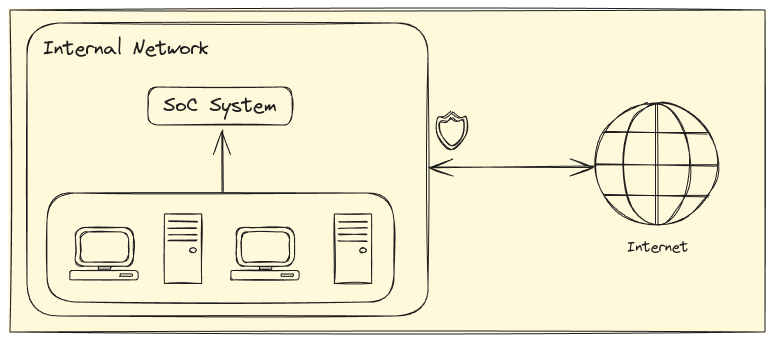
\includegraphics[width=1\textwidth]{src/assets/diagrams/soc-architecture-overview.png}
    \caption{High-Level Overview of SoC Architecture}
\end{figure}

% ----------------------- Integration with Existing Systems ----------------------- %
\section{Integration with Existing Systems}

Since implementing a SoC involves integrating with existing systems and processes, this section is about the challenges and best practices for seamless integration.

In our case, we will emulate a network environment with multiple endpoints, servers, and network devices to demonstrate the integration of the \glsxtrshort{soc}.

% ----------------------- Training and Skills Development ----------------------- %
\section{Training and Skills Development}

As is the case in every cybersecurity operation, training and skills development are crucial for the good operations of the \glsxtrshort{soc}.

This can include training on security tools, incident response procedures, threat intelligence analysis, and compliance requirements.

% ----------------------------------- SECTIONS (^) ----------------------------------- %

\setcounter{secnumdepth}{0} % Set the section counter to 0 so next section is not counted in toc
% ----------------------- Conclusion ----------------------- %
\section{Conclusion}
This chapter outlined the design process for a \glsxtrlong{soc}, covering requirements analysis, architectural design, system integration, and training.
The next chapter will demonstrate the \glsxtrshort{soc} implementation in an emulated environment.
